\chapter[Data transfers using everyday mobility: Taxonomy and state of the art]{Data transfers using everyday mobility:\\[-5pt] Taxonomy and state of the art}
\label{cha:state-of-the-art}

The emergence of wireless capabilities equipping an ever-growing range of mobile entities has led to various paradigms such as \acrfullpl{manet}, \acrfullpl{vanet}, \acrfullpl{wsn}, and \acrfullpl{dtn}. These paradigms enable the connectivity of a wide range of mobile entities in the context of various application scenarios ranging from transportation systems to sensing platforms. 

These different scenarios exploit entities that are mobile either by nature, such as humans or animals, or by conception, like vehicles and robots moving in challenging environments. The entities are equipped with storage capabilities, allowing them to store and carry data. They are also equipped with communication interfaces to forward data when the entities come in \textit{contact}\index{contact|bb}, \ie when they are in each others' communication ranges. While most of the approaches propose forwarding strategies to cope with the mobility of the entities, we focus on those that exploit the carrying phase resulting from the movements of the mobile entities. 

% We refer to this generic architecture as \textit{intermodal}\index{Intermodal|bb}, since multiple modes of data transportation are involved to route the data to its destination. 
In this chapter, we review and provide a comprehensive categorization of the \textit{existing strategies that leverage the existing mobility of entities to physically move data}. The movements of the entities provide an alternative transmission medium, as illustrated in Figure~\ref{fig:related-work}.

\begin{figure}[h]
    \vspace{-10pt}
    \centering
    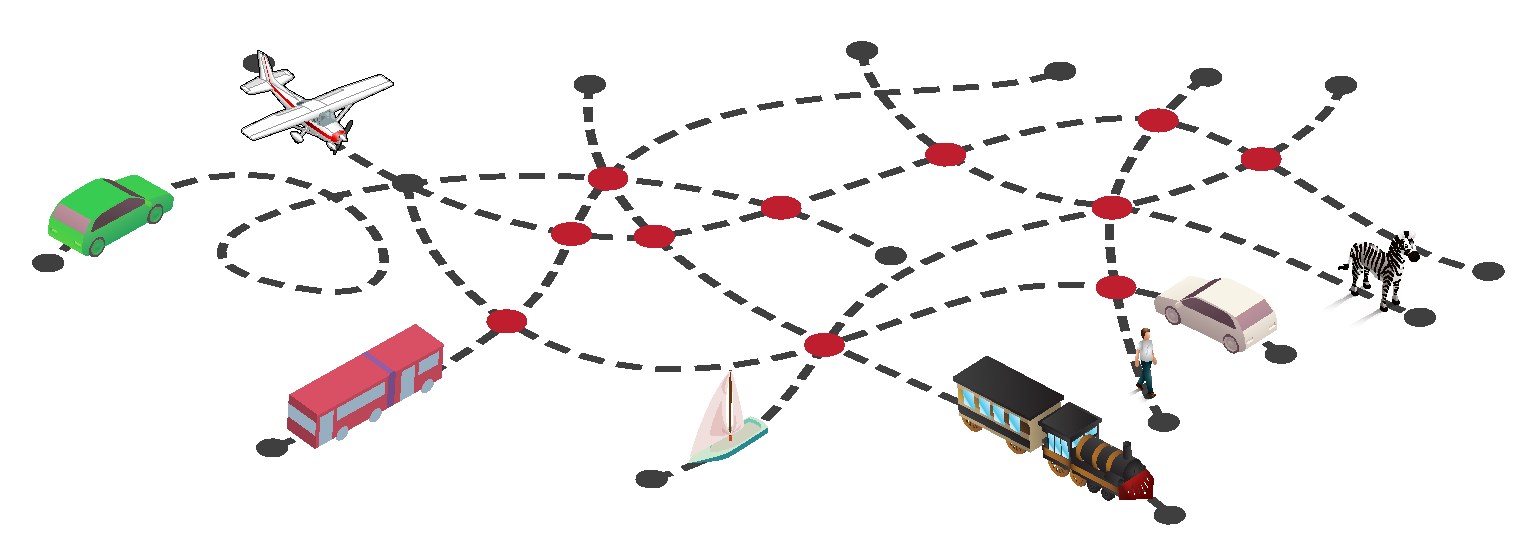
\includegraphics[width=0.55\textwidth]{figures/related-workv3.pdf}
    \vspace{-10pt}
    \caption{Alternative transmission medium based on the movements of entities.}
    \label{fig:related-work}
\end{figure}

% These entities help deliver data in environments with no infrastructure-based network available, or as a supplement or replacement to existing networks already deployed (\eg to extend their capacities). 

The idea of exploiting the mobility of different entities has been proposed in the context of various applications that do not require real-time communications. Some consider there is no data network available and entities are in charge of bringing network connectivity. Mobile entities can also be used in tandem with a conventional data network to extend the network coverage or capacity. In general, the applications rely on the following performance metrics to measure the efficiency of the data delivery:
\begin{itemize}
  \item \textit{Delivery delay}~---~the average delay to deliver the data from the sources to the destinations.
  \item \textit{Delivery rate}~---~the amount of data delivered to destinations per time unit.
  \item \textit{Delivery ratio}~---~the amount of data delivered to destinations divided by the total amount of data sent by sources that has been delivered.
  \item \textit{Energy efficiency}~---~the average amount of data delivered per unit energy consumption.
\end{itemize}  


\begin{figure}[!h]
\centering
\resizebox{\textwidth}{!}{%
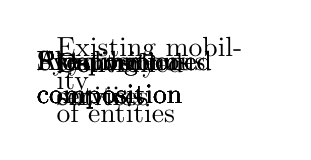
\begin{tikzpicture}[every tree node/.style={align=center,anchor=north},level 1/.style={level distance=1.5cm},level 2/.style={level distance=2cm},level 3/.style={level distance=2cm}]
\Tree [.\textbf{\large Data delivery} 
        [.{\textbf{Direct} data delivery\\Single entity}
            [.\node[text width=2.5cm]{Existing mobility\\of entities}; ] 
            [.\node[text width=2.5cm]{Controlled\\entities}; ]
            [.\node[text width=2.5cm]{Delivery\\services}; ] ] 
        [.{\textbf{Indirect} data delivery\\Multiple entities} 
            [.\node[text width=3cm]{Synchronous\\composition}; 
                [.\node[text width=3cm]{Pre-positioned\\composition}; ]
                [.\node[text width=3cm]{Floating\\composition}; ] ] 
            [.\node[text width=3cm]{Asynchronous\\composition}; 
                [.\node[text width=3cm]{Pre-positioned\\composition}; ]
                [.\node[text width=3cm]{Floating\\composition}; ] ] ] ]
\end{tikzpicture}}
\caption{Classification of the trajectory composition according to the type of data delivery.}
\label{fig:classification-survey}
\end{figure}

We represent the structure of the classification in Figure~\ref{fig:classification-survey}. Some works propose the use of a single entity to carry the data from its source all the way to the final destination. This results in a \textit{direct data delivery}, which we present in Section~\ref{sec:direct-delivery}. However, relying on a single entity is somehow limiting from the perspective of the expected benefits (\eg capacity or coverage). The idea of composing the trajectories of multiple mobile entities was thus introduced. According to this idea, the data follows a path consisting of multiple segments of trajectories, each followed by different mobile entities. This results in an \textit{indirect data delivery}, which we present in Section~\ref{sec:indirect-delivery}. Data is passed from one entity to another as a result of the forwarding when entities are in direct contact.

In the case of indirect data delivery, we choose to present the works that are the most relevant to this thesis. They propose different strategies for composing the trajectories of mobile entities. These strategies differ depending on the two following criteria:

\begin{itemize}
  
    \item The \textit{time} when composition should occur. The data is passed either \textit{synchronously} when two entities meet or buffered before passed \textit{asynchronously} to subsequent entities.  

    \item The \textit{location} where composition is performed. The location can be either \textit{pre-defined} or \textit{floating}. In the pre-defined case, the data is passed if the entities are in contact at specific locations. In the floating case, composition results of contacts between entities regardless where they are in contact.

\end{itemize}

The strategies proposed in the literature result of the combination of one of the instances of both previous criteria. 

% The simplest approach consists in using the movement of a single entity to eventually make the entire trip between the source(s) and the destination(s) of a data transfer. This approach is generally referred to as ``Direct delivery''\index{Direct delivery}. However, there are no guarantees on the actual delivery of data, as the movements of the entity are difficult to predict and do not necessarily match the source(s) and destination(s) of the data transfer. As a result, one entity is not enough to provide robust and reliable data transfers.

% Instead of using a single entity, \textit{concatenating} the movements of multiple entities to transport the data offers multiple paths to route the data, allowing to improve network performance (\eg delivery delay or ratio). The entities relay each other to transport the data from its source(s) to its destination(s) along a logical path and resulting in an indirect delivery. The concatenation of the movements corresponds to encounters between two entities when in each other's transmission range, that is when they are in \textit{contact}. They are the result of the opportunities to forward data when two entities come in contact. As a result, multiple concatenations of the movements of the entities are possible and their selection depends on the performance metrics to optimize. The movement concatenations are either synchronous or asynchronous, depending whether the entities directly forward the data or forward it via intermediate nodes. Synchronous concatenations are subjected to contacts, which that can happen anywhere between any two entities. They result from the decisions to either forward, replicate or keep the data. Conversely, asynchronous concatenations are the result of remote contacts between entities via intermediate nodes. The placement of stationary intermediate nodes or the movement of mobile ones induce the remote contacts between entities. Despite their uncontrollable movements, some entities share mobility patterns with common characteristics and concentrate in specific regions (\eg intersections in the case of vehicles). Since these regions have a high concentration of entities, they are more likely to encounter each other, creating potential concatenations of their movements. In this context, synchronous concatenation approaches benefit from the spatial distribution of the entities to geographically anchor the concatenation of their movements at specific locations with high entity concentrations. In the case of asynchronous concatenation, these locations correspond to the location of the stationary dedicated nodes.  

% In the following, we review both the direct and indirect delivery approaches.

% The contacts create opportunities to forward, resulting in different ways to concatenate the movements of the entities depending on the performance metrics to optimize.

% The entities can use this contact as an opportunity to forward the data they carry to one another. Indirect delivery approaches exploit the combination of the movements according to temporal and spatial dimensions. As contacts require encounters at the same time and location, the combination of movements is \textit{synchronous}. Conversely, approaches leverage dedicated nodes, either mobile or stationary to combine the movements of different entities in an \textit{asynchronous} manner. While the combination of the movements can happen anywhere, some approaches benefit from the spatial distribution of the entities to geographically anchor the combination of the movements of the entities at specific locations with high entity concentrations. In the case of asynchronous combination, these locations correspond to the location of the stationary dedicated nodes. 


\section{Direct data delivery}
\label{sec:direct-delivery}

In this section, we present the direct delivery strategies that exploit the movements of a single entity to carry data. We classify these strategies according to the degree of knowledge regarding the mobility of the carrying entity. 

Firstly, we consider the strategies using entities exhibiting random mobility. Although they eventually deliver the data they carry, the delivery delay can be excessively long, making the transfers unreliable and unfit for real-life applications. 

Having partial knowledge about the movements of the entities allows the deployment of applications that require performance guarantees, such as sensing platforms and systems to extend the connectivity of remote areas. 

Secondly, we consider the entities whose mobility is pre-calculated in advance. The related strategies and the related approaches to control their movements to transport the data. Controlling the movements of the entities provides better guarantees on the delivery delay and rate, which matches the requirements of sensing applications. 

Finally, we review the approaches that leverage third-party services such as postal services to transport data. These services allow the transfer of large amounts of data, resulting in a large capacity alternative medium for large-scale bulk data transfers.

\subsection{Existing mobility of entities}
\label{sec:direct-non-control}

\begin{wrapfigure}[11]{o}[0.7\marginparwidth]{5.5cm}
    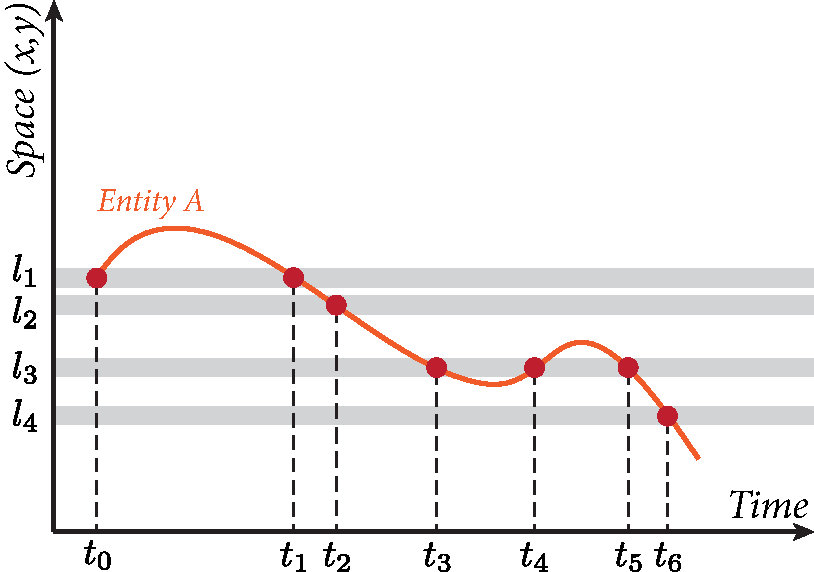
\includegraphics[width=5.3cm]{figures/dtn-direct-forwarding.pdf}
    \caption{Direct delivery using the existing movements of a single entity.}
    \label{fig:dtn-direct-forwarding}
\end{wrapfigure}
Several approaches rely on the existing movements of a single entity to transport the data in the context of delay-tolerant applications such as sensing platforms or periodic data transfers to bridge connectivity gaps in remote areas not covered by conventional data networks. The data is loaded in the storage of the mobile entity when it comes close to the source (\eg sensor nodes or gateway connected to a data network). As represented in Figure~\ref{fig:dtn-direct-forwarding}, the entity transports the data as part of its usual movements and unloads the data when it comes close to the destination (\eg sensor sink or gateway). Since only one copy of the data is carried, this approach does not consume many resources and has a minimum overhead. With no knowledge on the mobility of the entity, there are no guarantees on the expected delivery, which makes this strategy highly unreliable. However, some approaches exploit the knowledge of the mobility of the entity to deploy applications with stronger performance guarantees.

\paragraph{Random entity mobility.}
In the case of a random mobility, Grossglauer and Tse show how to use entities with unknown mobility to transport data instead of using traditional ad hoc networks where a wireless multi-hop path must always exist between the source and the destination~\cite{grossglauser2001mobility}. The direct delivery approach leads to better throughputs under large data loads compared to the ad hoc case, as most of the traffic carried by the entities in ad hoc networks is relayed traffic, which consumes both energy and bandwidth. However, using the mobility of the entities leads to high delays, as the entity carrying the data may take a long time before coming in contact with the destination. 

\paragraph{Large-scale sensing platforms.}
Large-scale sensing platforms can benefit from the random movements of entities to collect data from sensors scattered in an area, or even generate environmental data as part of their movements when equipped with sensors. The data is temporarily stored and carried by the entities and delivered to a central sensor sink when the entity moves close. The sensor sink aggregates the data to transfer it to remote servers using a conventional data network for long-term storage and analysis. Compared to ad hoc networks, this transmission model allows large power savings and higher bandwidth at the sensor nodes because the communications take place over short ranges, which reduces the power of the radios. 

Burrell~\etal study the deployment of sensor networks in vineyards to take effective decisions in the face of low temperatures, rain or frost. The authors relied on vineyard workers to transport the data from the sensors to the sink located in the farm~\cite{burrell2004vineyard}. SeNDT (Sensor Networking with Delay Tolerance) is a system for water pollution and noise monitoring at a lake in the center of the Republic of Ireland, which relies on sensors deployed around the lake~\cite{mcdonald2007sensor}. To collect the data, the authors mounted wireless devices on anglers' boats that they use to fish in the lake to collect sensor data as part of their movements on the lake. The data is then aggregated at a sink in the boathouse when the anglers return. The EMMA project aims at monitoring pollution using buses to generate location-based environmental data along their movements~\cite{lahde2007practical}. As part of their routes, the buses transport the data to stationary sinks placed in strategic locations, such as intersections. Using the existing movements of entities as part of sensing platforms to generate or collect sensing data avoids costly deployments to transmit the data through intermediate nodes and increases the lifetime of the sensor nodes by using short-range radios. However, such platforms must have loose constraints on the delivery rate and delay of the data as they rely on unpredictable movements of the entities.

With knowledge on the mobility patterns of the entities, DakNet leverages the bus schedules to provide Internet connectivity to remote regions of India and Cambodia~\cite{pentland2004daknet}. Equipped with mobile access points, the buses physically transport the data between Internet access points located in larger cities and rural kiosks located in the villages to exchange delay-tolerant data such as mail or land records. This provides an efficient low-cost alternative to expensive dialup 
\begin{wrapfigure}[9]{o}[0.7\marginparwidth]{5cm}
    \vspace{-10pt}
    \includegraphics[width=4.9cm]{figures/pigeon.jpg}
    \caption{A pigeon equipped with a backpack carrying an SD card.}
    \label{fig:pigeon}
\end{wrapfigure}
landlines or long-range radios. Compared to the previous approach, DakNet gives better guarantees because of the fixed schedule of the buses. A similar initiative was proposed by the Wizzy Digital Courier service to provide connectivity to access schools located in remote villages of South Africa~\cite{rabagliati2004wizzy}.

RFC 1149 specifies an experimental method to transmit IP datagrams using avian carriers, as represented in Figure~\ref{fig:pigeon}~\cite{rfc1149}. Although suited for very specific scenarios, this solution becomes infeasible in large-scale networks due to the high delay and low throughput of the transfer. Some implementations of the protocol lead to large losses (with over 55\% of lost datagrams) and variable delays of several hours when transporting the data over five kilometers.

While the endpoints of the pigeon route are pre-defined, its movements are random and lead to losses, making the transfer unreliable and unsuitable for the targeted applications. In the following, we overview the different approaches that leverage controllable entities to provide reliable data transport.

\clearpage
\subsection{Controlled entities}
\label{sec:direct-control}

\begin{wrapfigure}[11]{o}[0.7\marginparwidth]{5.5cm}
    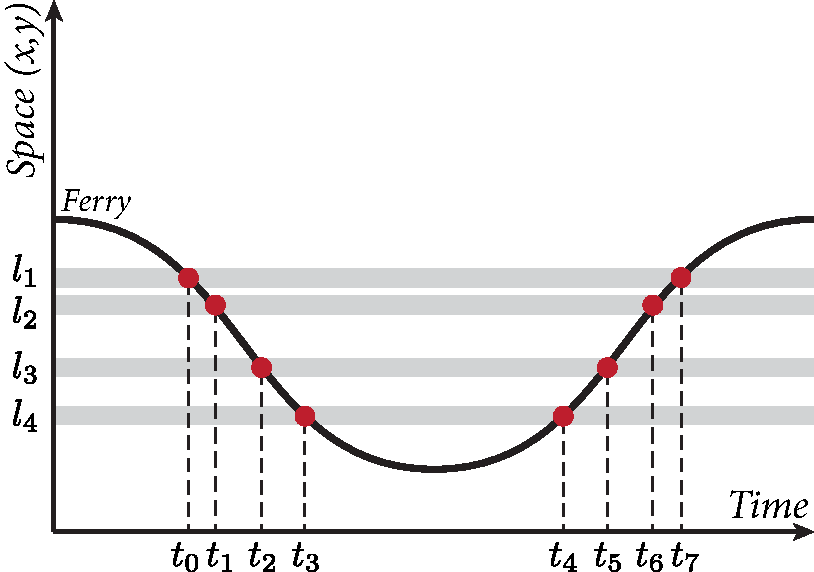
\includegraphics[width=5.3cm]{figures/dtn-direct-controlled-forwarding.pdf}
    \caption{Direct data delivery with a controllable entity.}
    \label{fig:dtn-direct-controlled-forwarding}
\end{wrapfigure}
Contrary to using the existing movements of entities, controlling their movements provides better performance guarantees, for instance on the delivery rate and delay of the data. Generally referred as ``ferries'' or ``robots'', these dedicated entities are generally used in sensor networks to provide communication capacity among the sensor nodes by picking up data from the source(s) and carrying it to the destination(s), as depicted in Figure~\ref{fig:dtn-direct-controlled-forwarding}. In this figure, a ferry periodically visit the nodes located at $l_1$, $l_2$, $l_3$, and $l_4$. An underlying challenge is to compute a route for the dedicated entity such that it visits all the nodes and optimizes performance metrics (\eg average delivery delay and rate). In the work we review, the nodes generate data traffic (uniform or not), which results in different bandwidth requirements that the dedicated entity has to satisfy. Otherwise, the data generated at the nodes accumulates to a point where it is dropped in case of limited buffer capacity.

\paragraph{Message ferry.}
In the initial message ferry work, Zhao \etal proposed an algorithm to compute the ferry route of a single ferry such that it minimizes the average delivery delay of the data generated uniformly by a collection of stationary nodes~\cite{zhao2003message}. The algorithm first creates a route using local optimization techniques for the \acrfull{tsp} (2H-opt) that minimizes the average delay for all traffic generated by the nodes. Second, the algorithm extends the original route to meet the bandwidth requirements of the nodes. While this technique works well with equal node bandwidth requirements, it does not adapt to unequal ones. 

\paragraph{Unequal bandwidth requirements at the entities.}
With unequal bandwidth requirements, Mansy \etal propose to use the deficit round-robin technique to decide which node to visit next depending on the visit history and the last meeting with the ferry~\cite{mansy2011deficit}. With this approach, nodes with higher data rates get better chances to be visited by the ferry. Tirta \etal propose to decrease the delay of the ferry route by visiting fewer nodes using the ad hoc connectivity of the nodes to form clusters~\cite{tirta2004efficient}. The ferry only visits one node per cluster, the \textit{cluster head}, which aggregates and distributes the data from and to the other nodes of the cluster. The authors focus on the impact of different route schedules on the buffer size of the cluster head, which sees a large load of messages to aggregate and distribute. The authors show that scheduling the visits of the ferry to minimizing its movements reduces the energy consumption of the ferry. However, scheduling the visits of the ferry at the cluster heads according to the data rate aggregated at the cluster heads leads to better delivery delays.

\paragraph{Multiple controllable entities.}
Adding more controllable entities to collect the data of the nodes increases the cost, but also improves the network capacity and overall performance, as the entities can cover larger distances, handle more traffic load, and provide better reliability in case of failure. Zhao \etal propose two different techniques to directly deliver data among the nodes using multiple message ferries~\cite{zhao2005controlling}. The first technique consists in designing a single route using the same heuristic as followed by all the ferries with the same speed and different timings, allowing each node to communicate with all the ferries~\cite{zhao2003message}. The second technique is more complex and consists in designing multiple routes followed by the ferries instead of a single route. Since the data is not relayed by the ferries, each route must accommodate all the bandwidth requirements of the node visited by the ferry on the route. The authors propose a greedy heuristic that assigns nodes to ferries and balances the traffic load among the routes by shortening or extending them such that the estimated weighted delay of the data traffic among the nodes is minimized. 

More recently, pigeon networks introduced \textit{pigeons} that act as ferries between a ``home host'' and ``foreign hosts'' on dedicated routes~\cite{zhou2013minimizing}. There are no data exchanges between the ferries, so each route must accommodate the requirements of every foreign host they visit. The authors propose an exact optimization technique to design the routes of the pigeons such that they minimizes the average delay of the generated data. This technique is optimal for small-scale networks but becomes intractable for larger networks. To make the problem tractable, they propose a geographical partitioning-based heuristic that relies on the divide-and-conquer idea to design the pigeon route. The authors show that the resulting route yields lower delays compared to the non-partitioning strategy used in the route design of the message ferry work.

\paragraph{Real-world deployments.}
Several projects have studied and deployed controllable entities in real-life settings in the context of sensing platforms. Tekdas~\etal deployed a small sensor network with robots to measure the energy savings brought by the addition of the robots~\cite{tekdas2009using}. With robots assigned to different routes using the $k$-\acrshort{tsp} heuristic, which finds $k$ tours where the largest of the $k$ tours is minimized, they showed significant energy savings at the sensor nodes from 1mW in tradition ad hoc to 0.003mW with the robots. Since the robots come close to the sensor nodes, they require limited transmission power and fewer transmission attempts, which decreases the overall energy consumption. 

\paragraph{Underwater networks.}
Underwater networks of sensors deployed in the oceans for long-term environmental monitoring or surveillance also leverage robots to collect sensor data~\cite{partan2007survey,akyildiz2005underwater,dunbabin2006data}. Because of the cost of the underwater sensor nodes and the extent of the areas to monitor, the deployment of underwater sensor networks is generally sparse, making it impossible to form an unpartitioned ad hoc network. Robots or \acrfullpl{auv} transport sensor data between the sensor nodes in the partitions. These networks differ from terrestrial sensor networks because of the acoustic channel shared between the communications among the sensors and the \acrshortpl{auv}, and the navigation system of the \acrshortpl{auv}. This twofold utilization of the medium creates contentions, limiting its use. The \acrshortpl{auv} use visual odometry to travel to the next sensor node and collect its data. The \acrshortpl{auv} then send via a high-bitrate channel the data collected from the underwater sensors to buoys acting as sinks.

Using controllable entities to enable the communication between static nodes gives better delivery delays and rates, as the route followed by the entity is specifically designed to optimize these metrics. In the following, we review the approaches that use existing delivery services to transport the data instead of controlling the mobility of entities. These approaches rely on entities already operated and managed by the delivery services.

\subsection{Delivery services}
\label{sec:thrid-party-services}

% Contrary to the previous approaches that target sensing platforms or remote transfers to bridge the connectivity gap between remote regions, the approaches we review here leverage third-parties to transport data. Commonly referred as \textit{SneakerNet}\index{SneakerNet|bb}~\cite{patterson2003conversation}, these approaches control the endpoints of the data transfers. They create an alternative transmission medium to offload data from infrastructure-based networks. Offloading was used during the Cold War by diplomats to exchange suitcases with one-time pads printed on tapes to encode the real-time communications between Washington and Moscow~\cite{kahn1974codebreakers}. While offloading can create a secure channel, it also has a high bandwidth potential, as stated by Andrew Tanenbaum\index{Tanenbaum|bb}~\cite{tanenbaum2003computer}:
% \begin{quote}
%     \textit{Never underestimate the bandwidth of a station wagon full of tapes hurtling down the highway.}
% \end{quote}

\begin{wrapfigure}[10]{o}[0.7\marginparwidth]{5.5cm}
    \vspace{-10pt}
    \centering
    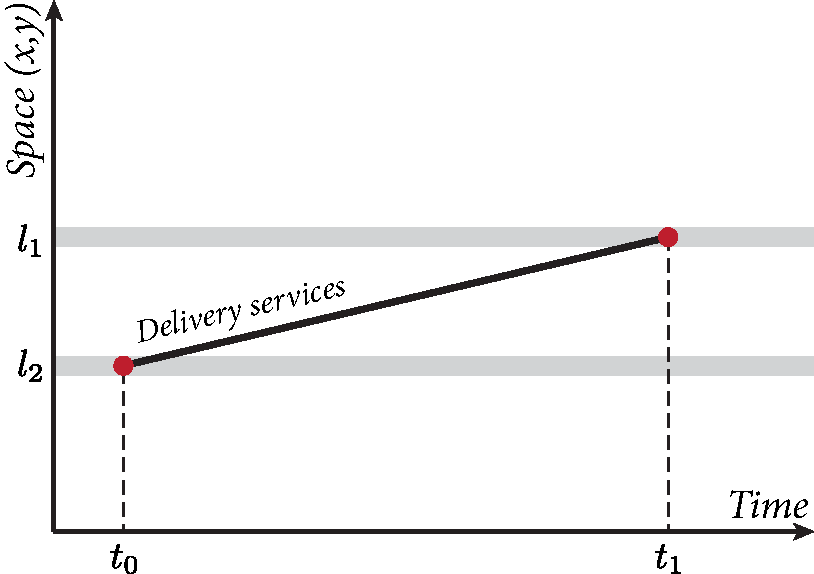
\includegraphics[width=5.3cm]{figures/dtn-direct-delivery.pdf}
    \caption{Direct data delivery using delivery services.}
    \label{fig:dtn-direct-delivery}
\end{wrapfigure}
Delivery services (\eg USPS, La Poste, FedEx, or UPS) provide an alternative mean to transport data by shipping hard drives and disks over long distances, as they avoid deploying and maintaining costly conventional data networks. Delivery services target delay-tolerant transfers and provide guarantees on the delivery date and shipping cost of the parcels. We represent their use in Figure~\ref{fig:dtn-direct-delivery} where the data is transported from location $l_1$ to location $l_2$.

Wang~\etal proposed Postmanet, a generic system that complements the Internet and provides connectivity to areas in rural regions using postal services~\cite{wang2004turning}. The data is copied on DVDs and shipped in parcels to remote Postmanet routers that act as gateways similar to rural kiosks, which, in turn, put the received data at disposal to the remote users (\eg email or land records). The authors overview different routing strategies to ship the data, including direct shipping between users. Since the other strategies rely on intermediate servers to dispatch the data, we will review them in Section~\ref{sec:indirect-async-anchored} where we review the indirect delivery approaches. 

\begin{wrapfigure}[9]{o}[0.7\marginparwidth]{4.4cm}
    \centering
    \vspace{-15pt}
    \includegraphics[width=3cm]{figures/Snowball.png}
    \caption{Amazon Snowball.\index{Amazon Web Services (AWS)!Snowball}}
    \label{fig:snowball}
\end{wrapfigure}
Laoutaris~\etal compared the cost of sending data using postal services with the cost of sending the same amount of data through a conventional data network, as content providers operating several datacenters would do~\cite{laoutaris2009delay,laoutaris2013delay}. Such data transfers are currently serviced by expensive dedicated networks (\eg Large Hardon Collider Computing Grid) or by postal services. The authors exploit intermediary storage in transit \acrfullpl{isp} to temporarily buffer the data and send it during off-peak hours when the costs to transmit data are low. The authors found that it is less expensive to use the postal services for individual shipments that occasionally happen (\eg short-lived transfers). However, in the case of a constant flow of data to transfer, they show that shipping data is more expensive than sending it through an \acrshort{isp} using the intermediate storage the authors propose to use.

\paragraph{Commercial applications using delivery services.}
Many commercial applications rely on postal services to exchange content with their customers. As an example, Netflix\index{Netflix} offers a DVD rental service to its customers\footnote{\url{http://dvd.netflix.com/}} which allows them to rent DVDs and receive them in the mail. Netflix' customers may keep a DVD as long as they want, and must return it before renting another DVD. With this service, Netflix currently distributes more than 1.5~million DVDs a day\footnote{\url{ http://ir.netflix.com}}, accounting for a total aggregate bandwidth of more than 650 Gbps. 
% http://files.shareholder.com/downloads/NFLX/182838532x0x102020/5a5dc220-6f8b-4704-a380-2c81a3a37958/factsheet.pdf

Large cloud providers offer services to allow their customers to ship physical media of their data to be uploaded to remote cloud storage (\eg
\acrshort{aws} Import/Export\index{Amazon Web Services (AWS)!Import/Export}\footnote{\url{http://aws.amazon.com/importexport}}, 
Microsoft Import/Export Service\footnote{\url{http://azure.microsoft.com/en-us/documentation/articles/storage-import-export-service/}} and more recently 
Google Offline Disk Import\footnote{\url{https://cloud.google.com/storage/docs/offline-media-import-export}}). AWS launched the Amazon Snowball\index{Amazon Web Services (AWS)!Snowball} (shown in Figure~\ref{fig:snowball}) is a portable ready-to-be-shipped appliance with a storage capacity of 50~TB that aims to accommodate transfers of several Petabytes (using multiple Snowball) to \acrshort{aws} servers. Amazon compares this solution with transfers on common Internet connections and shows that it takes approximately a week to transfer 50~TB via a 1G connection, or to ship a  Snowball with the same amount of data. Therefore, this solution exemplifies the potential of physically transferring data for massive data offloading.

% With this appliance, Amazon customers trade speed for money, as renting a Snowball costs \$200 plus the shipping costs. Comparatively, leasing a dedicated line from a Tier 1 ISP (\eg Level 3) costs about \$1~-~\$2 per Mbps for a 10G port, which rounds up to \$10,000 for a fully utilized 10G port (including collocation and equipment leasing costs)\footnote{\url{http://drpeering.net/white-papers/Internet-Transit-Pricing-Historical-And-Projected.php}}. Therefore, as noted by Laoutaris \etal~\cite{laoutaris2009delay}, leasing an Amazon Snowball for a single transfer is more profitable than leasing a dedicated line for similar resulting bandwidth.

% \begin{table}[h]
%     \centering
%     \begin{tabular}{|c|c|c|c|c|}
%         \hline
%          & \multicolumn{4}{c|}{Internet connection speed} \\
%         \hline
%         Utilization & 1Gbps & 500Mbps & 300Mbps & 150Mbps\\
%         \hline
%         25\% & 19 & 38 & 63 & 126 \\
%         \hline
%         50\% & 9 & 19 & 32 & 63 \\
%         \hline
%         75\% & 6 & 13 & 21 & 42 \\
%         \hline
%     \end{tabular}
%     \caption{\textit{How fast is that truck full of drives?}~---~Numbers of days to transfer 50~TB via the Internet at typical utilizations. The table appeared on slides from Amazon Web Services.} 
%     % \footnote{\url{http://www.slideshare.net/AmazonWebServices/aws-october-webinar-series-introducing-aws-import-export-snowball}}.}
%     \label{tab:truck-full-of-drives}
% \end{table}


\section{Indirect data delivery}
\label{sec:indirect-delivery}

As we have seen in the previous section, relying on the existing movements of a single entity to transport the data limits the expected performance of the resulting transfers, in terms of the delivery delay and rate. Instead of one entity, one can \textit{compose} the trajectories of multiple entities to transport the data to its destination. Composing the trajectories of entities gives the opportunity to route the data on multiple paths, thus increasing the resulting capacity and reliability of the data transfers. As we have mentioned in the introduction of this chapter, we classify the different strategies for composing the trajectories of entities depending on the time and location of the composition. 

Firstly, we review the strategies that rely on the synchronous composition of the trajectories of entities. In this case, the data is then passed from one entity to another whenever two entities come in contact. The different strategies we review propose more of less elaborated control planes to decide whether to forward, replicate, or keep the data during a contact to optimize the performance of the resulting data transfers.

Secondly, we review the strategies that rely on a dedicated infrastructure that consists of either stationary or mobile nodes with controlled mobility to asynchronously compose the trajectories of the entities. This infrastructure mitigates the effects of the partial knowledge of the movements of the entities and allows efficient compositions of the movements to improve the performance of the data transfers, in terms of delivery delay and rate. 

% This combination can be synchronous or not and can happen at specific locations or not. The data is then relayed from one entity to another whenever two entities encounter or come in contact with each other's transmission range. When in contact, the entities decide whether to forward the data or not to the other entity. The entities may also decide to replicate the data, thus increasing the number of possible paths to the destination. While replication seems appealing to increase the chances to deliver the data in less time, it requires more node resources (\eg storage and energy) to buffer and transmit the additional copies of the data. However, these decisions are difficult to make when the mobility of the entities is not well-known. Approaches proposed to introduce non-randomness by deploying a dedicated infrastructure to support the data transport. This infrastructure consists of mobile or stationary nodes that \textit{asynchronously} relay the data between entities. In this section, we review the different approaches that leverage synchronous forwarding between entities in contact and asynchronous forwarding with support infrastructure.

\subsection{Synchronous composition of the trajectories}
\label{sec:indirect-sync}

If the data is passed in a synchronous way, the two mobile entities involved in the composition of their trajectories are required to be in contact at the same time. As a result, the data follows a route that consists of the successive compositions of the trajectories of the entities that physically carry the data towards its destination. This approach is commonly referred to as \textit{mobility-assisted forwarding}, or also as \textit{store-carry-and-forward}. The work we review in this section proposes different control plane approaches to make the forwarding decisions over contacts. Instead of using straightforward decisions based on a local control plane, the approaches that leverage a global control plane make more informed and efficient forwarding decisions to improve the performance of the data transfers. 

While the contacts can occur anywhere, only few should be considered to compose the trajectories of the entities. Some strategies only consider the compositions that result of the contacts occurring in specific pre-defined areas. These areas correspond to locations with higher densities of entities with more contact opportunities than the other locations with lower densities. Routing data between these areas enables better control of the forwarding and requires fewer replications to deliver the data.

In the following, we present the strategies that transfer the data over synchronous compositions of the trajectories of entities either with floating compositions or at pre-defined locations.

% With synchronous combinations, the data follows a route that results from the successive combinations of the movements of the entities that physically carry the data towards its destination. This approach is commonly referred to as \textit{mobility-assisted forwarding}, or also as \textit{store-carry-and-forward}. The work we review in this section proposes different control plane approaches to make the forwarding decisions over contacts. Instead of using straightforward decisions based on a local control plane\index{Control plane}, the approaches that leverage a global control plane make more informed and efficient forwarding decisions, thus enhancing the network performance. With a global control plane, some approaches restrict the forwarding decisions to geo-anchored locations with higher densities of entities. Having more concentrated contact opportunities increases the chances to make the right forwarding decisions. In a first part, we review the approaches that do not restrict the forwarding decisions to any specific locations and in a second part, we review the approaches that leverage forwarding decisions geo-anchored at specific locations.


\subsubsection{Floating composition}
\label{sec:indirect-sync-non-anchored}
% DTN routing

\begin{wrapfigure}[10]{o}[0.7\marginparwidth]{5.5cm}
    \vspace{-10pt}
    \centering
    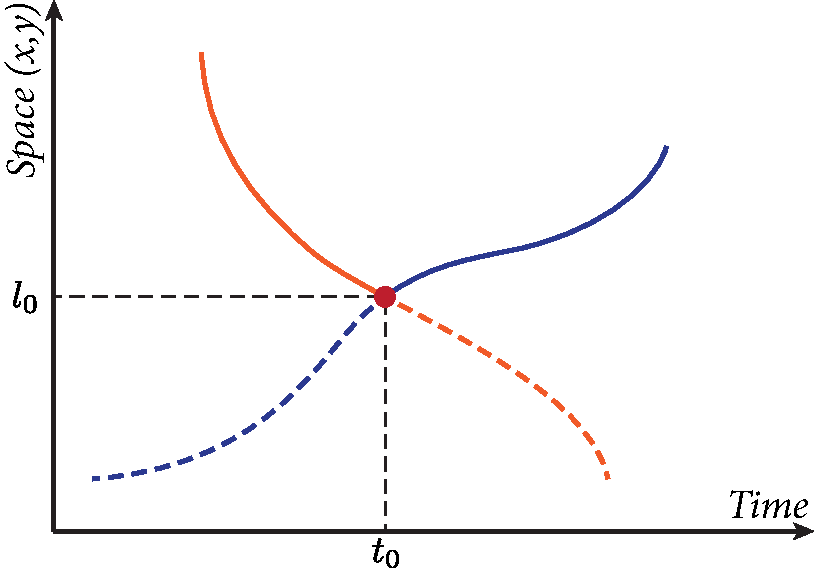
\includegraphics[width=5.3cm]{figures/dtn-indirect-sync-nongeo.pdf}
    \caption{Indirect synchronous floating composition between two entities.}
    \label{fig:dtn-indirect-sync-nongeo}
\end{wrapfigure}
When two entities come in contact at the same time and location, it creates an opportunity to compose their trajectories and bring the data closer (in time) to its destination. We represent the floating composition in Figure~\ref{fig:dtn-indirect-sync-nongeo} where the data is passed from entity $B$ to entity $A$. During a contact, the two entities can forward, replicate, or keep the data they carry. In this section, we review the different strategies to synchronously compose the trajectories of entities. The applications envisaged with these strategies must tolerate delayed deliveries. They range from sensor networks to vehicular networks and battlefield communications.

\paragraph{No control plane.}
With no control plane, the entities compose their trajectories with any other entities they encounter by replicating the data they carry. This is how the epidemic protocol works by disseminating the data~\cite{vahdat2000epidemic}. Every intermediate entity that receives the data replicates it to all its neighbors and so on. With this approach, the data is certain to be delivered with the minimum delay at its destination, as one of the copies follows the shortest route between the source and the destination. However, under limited resources, including buffer storage, this strategy is not efficient as it creates an exponential number of copies of the data and fills the buffers of the entities.

Originally proposed in the context of sensing platforms, the data \acrshort{mule} architecture leverages the movements of entities to collect data from sensors scattered in a sparse area and deliver it to access points~\cite{shah2003data}. To improve the system performance, the \acrshortpl{mule} can communicate with each other to either form an ad hoc multi-hop \acrshort{mule} network or to compose their movements and disseminate the data when in contact. CarTel~\cite{hull2006cartel} and BikeNet~\cite{eisenman2009bikenet} have both implemented the data \acrshort{mule} architecture to generate sensing data using sensors mounted on vehicles and bikes equipped with sensors, respectively. Note that, in both works, the dissemination protocol was not implemented and was instead replaced by a direct delivery approach.

The Infostation model presents a data \acrshort{mule} application where mobile entities connect to Infostations that act as access points distributed over a geographical area~\cite{goodman1997infostations}. When in the vicinity of an Infostation, the entities transmit at very high rates, thus trading connectivity for capacity. With the Shared Wireless Infostation Model, Small and Haas enhanced the Infostation model with the epidemic routing in the context of whale monitoring with radio-tagged whales that continuously collect biological and environmental data~\cite{small2003shared}. The data collected by the whales is then transmitted when the whales surface to buoys that act as Infostations. The epidemic protocol is used to exchange monitoring data when the whales are grouped together. Since the epidemic protocol generates a large number of replicas, the data accumulates at the buffers, resulting in buffer overflows and data drops. To limit the number of copies of the same file in the network, the authors use an infectious disease model that ``infects'' the whale with a data according to a given probability, if not already infected. This probability is chosen such that it is equal to the probability that the data will be offloaded within a target duration since its generation. 

\paragraph{Maintaining a local control plane.}
Subsequent approaches proposed a local control plane to improve the performance epidemic protocol and limit the excessive usage of the resources. The Spray-and-Wait protocol bounds the number of copies to send per data using two phases~\cite{spyropoulos2005spray}. In the ``spray'' phase, a given number of copies are transmitted from the source to other entities that act as relays. In ``wait'' phase, the relays with a copy of the data wait to encounter the destination of the data. The Spray-and-Focus protocol~\cite{spyropoulos2007spray} uses the same ``spray'' phase as~\cite{spyropoulos2005spray}, followed by a ``focus'' phase where the copies can be forwarded to other relays to help maximize a utility function (\eg delivery delay).

Other approaches proposed a more elaborated local control plane where each entity records its encounters with the other entities. This is the case of the meets and visits protocol, where each entity learns the frequency of meetings between entities and visits to certain locations in order to estimate the likelihood of forwarding the data to other entities~\cite{burns2005mv}. BUBBLE is a protocol that leverages the communities formed by entities such as humans to select high centrality entities (the most popular ones) and members of the community of the destination entity as relays~\cite{hui2011bubble}. To this end, the authors rely on distributed approach where each entity detects the communities and approximates the centrality of the other entities they encounter. Other protocols such as GeOpps~\cite{leontiadis2007geopps} and GeoSpray~\cite{soares2014geospray} exploit the geographical information of navigation systems of vehicles to forward the data towards its destination and minimize the estimated time of delivery of the data.

\paragraph{Maintaining a global control plane.}
A global control plane allows every entity to have the same view of the network to make better decisions when composing their trajectories. To this end, the strategies with a global control plane exchange historic encounter information.  PROPHET leverages the control information of the histories of all encounters to estimate a delivery predictability of the data~\cite{lindgren2003probabilistic}. It indicates how likely an entity is to deliver a data to a destination. The data is then forwarded to the entity with the highest estimate. RAPID is another routing protocol that treats routing as a resource allocation protocols~\cite{balasubramanian2010replication}. It determines the degree of replication of a message by estimating the suitability of a contact to optimize specific metrics (\eg minimize the average delivery delay) according to a replication utility. To this end, the entities exchange network state information (\eg expected meeting times with entities and past encounters) and acknowledgments among the entities. MaxProp is a routing protocol for delay tolerant networks designed in the context of the UMass DieselNet testbed~\cite{burgess2006maxprop}. DieselNet is a vehicular network that consists of 40 buses equipped with WiFi capabilities serving the surrounding area of UMass Amherst campus. With MaxProp, the data forwarding results of local decisions made by each bus according to a delivery likelihood estimation based on the history information about the past meetings with other buses. While this strategy allows having a global shared control plane, it requires exchanging large amounts of control information for large networks. Additionally, the shared view of the network is not consistent, as the control information takes time to be propagated in the network.

\paragraph{Discarding the remaining copies of the data.}
One of the problems with the previous approaches is to discard the remaining copies of the data once successfully delivered. Some approaches flood delete-lists to discard the remaining copies of the delivered data. This is the case of ZebraNet, a platform to monitor zebra wildlife in Kenya and track their location history logged in collars~\cite{juang2002energy}. The data logged in the collars is reported when the zebras come in the range of base stations, which are either fixed or mobile, handheld by the researchers when they occasionally drive-by or fly-by to collect the data from the animals. The authors used the epidemic protocol to transmit the data from one zebra to another and increase the chances the data will be delivered to a base station. The delete-lists are updated with a gossip protocol whenever two zebras are in contact. Similarly, MaxProp~\cite{burgess2006maxprop} and RAPID~\cite{balasubramanian2010replication} both propagate acknowledgments in the network to remove stale data from the buffers and free some space to avoid buffer overflows. 

The addition of a control plane helps to increase the performance of the data transfer resulting from the composition of the trajectories of the entities. The control plane gives information on how likely an entity is likely to bring the data closer to its destination. However, in real life, the composition can happen anywhere, but only the contacts that happen in a few specific areas are worth considering to improve the performance of the transfers~\cite{kang2004extracting,sarafijanovic2006island}. The strategies we review in the following restrict the compositions of the trajectories to pre-defined locations.

\clearpage
\subsubsection{Composition at pre-defined locations}
\label{sec:indirect-sync-anchored}

\begin{wrapfigure}[10]{o}[0.7\marginparwidth]{5.5cm}
    \vspace{-23pt}
    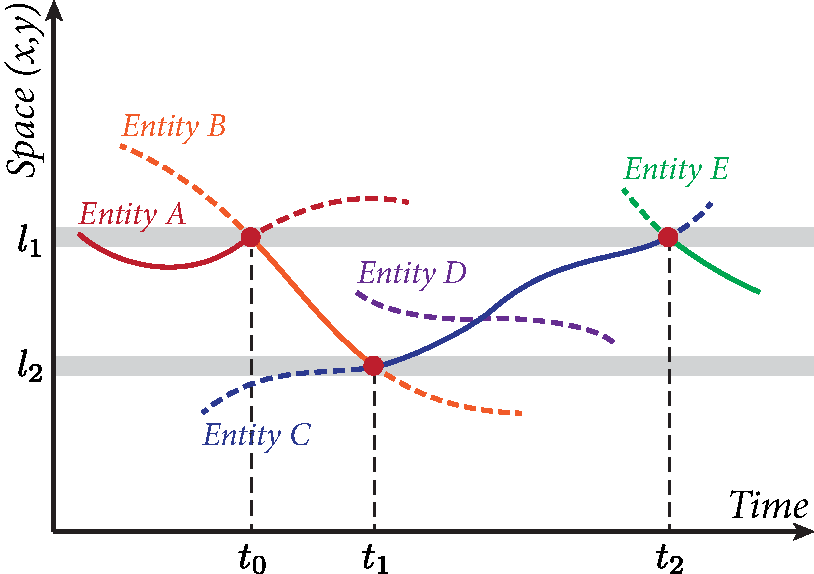
\includegraphics[width=5.3cm]{figures/dtn-indirect-sync-geo.pdf}
    \caption{Indirect synchronous composition between two entities at pre-defined locations.}
    \label{fig:dtn-indirect-sync-geo}
\end{wrapfigure}
Instead of composing the trajectories of the entities anywhere in the geographic area, some strategies only allow the composition at pre-defined locations, as shown in Figure~\ref{fig:dtn-indirect-sync-geo}. In this case, the composition of trajectories can only happen at locations $l_1$ and $l_2$. These strategies exploit the high density of entities and their movement patterns in these areas where the contacts between the entities are more likely to happen (\eg road intersections). These areas have been exploited by context- and location-aware services such as digital graffiti~\cite{carter2004digital} and floating content~\cite{ott2011floating} to anchor content at specific locations. 

In the case of data transfer, the use of these concentrated areas enables a finer control of the routing strategies to limit the number of replications needed when forwarding a data from an area to another. Most of the approaches we review in this section leverage a logical representation of the system with an overlay graph to route the data in the areas on the shortest path. The nodes of the overlay correspond to the areas with high densities of entities and the links represent the movements of the entities between the nodes. 

\paragraph{Determining the locations where to compose the entity trajectories.}
An underlying problem related to this approach is to determine the locations with high densities of entities. In an urban vehicular setting, they correspond to intersections at junctions and traffic lights. In the context of \acrshortpl{vanet}, LOUVRE~\cite{lee2008louvre} and GyTAR~\cite{jerbi2009towards} build an overlay network on top of intersections (``landmarks'' in the case of LOUVRE) where vehicles are connected to each other. When the vehicles come to the intersections, they forward the data over overlay links representing the \acrshort{vanet} multi-hop path between two adjacent intersections. Similarly, Tan~\etal uses the movements of vehicles traveling a transportation network to create a ``vehicular backbone network''~\cite{tan2014vehicular}. The vehicles perform ``wireless switching'' when they are in contact at intersections or on dual-way roads when vehicles travel in opposite directions. Sarafijanovic-Djukic \etal characterize the locations with high entity densities as ``concentration points'' (CP)~\cite{sarafijanovic2006island}. Using real-life traces, the authors defined CPs as areas with at least 5\% of the vehicles per day. In the context of multiple message ferries following different routes and creating a communication medium among static nodes, Zhao \etal propose to pass the data between the ferries at intersecting points of their routes~\cite{zhao2005controlling}. In this case, the ferry routes must be synchronized for the ferries to come in contact regularly. Ker{\"a}nen and Ott propose to transport data between airports using the smartphones of the airline passengers~\cite{keranen2009dtn}. The authors rely on the scheduled flight connections at airports to compose the trajectories of the passengers. 

\paragraph{Maintaining a global view of the network state.}
The entities must have a consistent and up-to-date view of the overlay network to know where and how to forward the data. There are two approaches to knowing this information. The first approach consists in assuming a low-bandwidth control channel to exchange the control messages that have low overhead. This is the case of Tan \etal that uses this control channel to have the latest estimation of the overlay link metrics~\cite{tan2014vehicular}. In the ferry work, Zhao \etal use this control channel to compute the intersecting routes of the ferries in an offline manner~\cite{zhao2005controlling}. The second approach leverages an in-band distributed approach. In~\cite{sarafijanovic2006island}, the entities distribute the information about the overlay using a collaborative graph discovery protocol. While this method does not provide an up-to-date information, it avoids relying on signals from the environment. LOUVRE and GyTAR rely on a peer-to-peer density discovery to populate link state table of the overlay nodes with the density information. However, in the case of a large-scale network such as the airline network proposed by Ker{\"a}nen and Ott, the entities cannot maintain information about all the links in the overlay. The authors argue that epidemic protocols that replicate the data are more suited for this case to forward the data~\cite{keranen2009dtn}.

\paragraph{Forwarding data when in the specific areas.}
With the information about the overlay, the entities can make forwarding decisions in the pre-determined areas to route the data on the shortest path to its destination. With no information on the future trajectories of the entities, \cite{sarafijanovic2006island} propose to replicate the data to multiple entities to increase the chances that at least one will arrive at the next overlay node. Once the data has reached the next entity, an acknowledgment is broadcasted to the previous entity to discard the remaining copies of the data. Tan \etal forward the data to minimize the delivery delay of the data and guarantee the fairness among the flows~\cite{tan2014vehicular}. When two vehicles encounter, they choose the data flow and overlay link that are the least used of those available and the pre-allocated ones. In LOUVRE and GyTAR, the routing protocol uses the well-known Dijkstra algorithm to use the link state tables and forward the data on the overlay links with the highest density of entities~\cite{lee2008louvre,jerbi2009towards}.

Using the spatial distribution of the entities to restrict the composition of the trajectories to areas where entities concentrate allows better control of the forwarding. The logical representation of the network makes the allocation of the data transfers possible and improves the performance of the resulting data transfer compared to the floating case. In the following, we review the strategies that leverage a dedicated infrastructure that temporarily buffer the data to asynchronously compose the trajectories of the entities. As a result, contrary to the synchronous case, they do not have to encounter at the same time and place to pass the data.


\subsection{Asynchronous composition of the trajectories}
\label{sec:indirect-async}

While restricting the compositions of the entity movements to specific locations can improve the forwarding decisions, the movements of the entities between the locations can be unpredictable. To overcome the randomness, other approaches propose to rely on a dedicated infrastructure with intermediate nodes, either mobile or stationary, that temporarily buffer the data carried by the entities before passing it to subsequent entities. In this case, direct contacts between the entities are not required, allowing the data to be passed asynchronously. 

The use of mobile intermediate nodes, such as ferries or robots, allows remote entities to communicate together, even if their trajectories do not intersect. These nodes follow pre-scheduled routes to bridge the trajectories of distant entities. In this case, the composition of the distant entities is asynchronous and floating.

Stationary intermediate nodes, such as offloading spots or throwboxes, enable the communication between two entities whose trajectories do not necessarily intersect at the same time. As a result, these nodes are pre-positioned at specific locations frequently visited by the entities. In this case, the composition of the entities is asynchronous and happens at pre-defined locations.

In the following, we review the strategies that rely on intermediate nodes to support the data transport. In the first part, we review the strategies with mobile nodes and those with stationary nodes in the second part.

\subsubsection{Floating composition}
\label{sec:indirect-async-non-anchored}

% - choose the next node to visit to satisfy the node requirements (dynamic)
% - Communication with the nodes
% - distribution of the global state (distributed vs central)
% - Using multiple message ferries

\begin{wrapfigure}[9]{o}[0.7\marginparwidth]{5.5cm}
    \vspace{-37pt}
    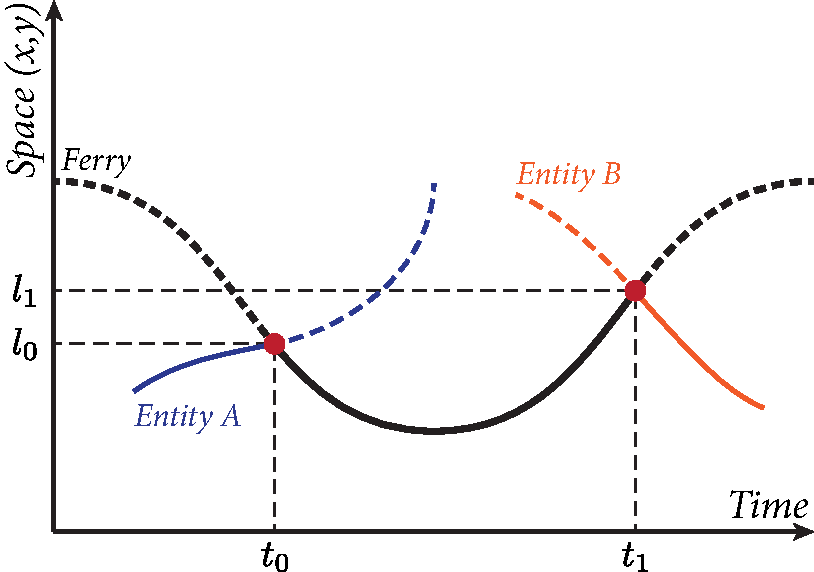
\includegraphics[width=5.3cm]{figures/dtn-indirect-async-nongeo.pdf}
    \caption{Indirect asynchronous floating composition between two entities using a \textit{ferry}.}
    \label{fig:dtn-indirect-async-nongeo}
\end{wrapfigure}
Mobile intermediate nodes, such as ferries or robots enable the composition of the trajectories of remote entities together. As a result, the data is passed asynchronously between the entities. In Figure~\ref{fig:dtn-indirect-async-nongeo}, we represent the asynchronous composition of the trajectories of entities $A$ and $B$ using a ferry that encounters the entities. These intermediate nodes enhance the capacity of the mobile networks by providing more opportunities to compose the movements of the mobile entities. As a result, they provide an on-demand data transport service to serve the requests to transfer data of the entities.

\paragraph{Determining the next entity to visit.}
With mobile entities, the ferries must dynamically determine the next entity to serve to optimize given metrics (\eg bandwidth requirements of the entities). In the \acrfull{fimf} proposed by Zhao \etal, the ferry follows a default route and receives requests from the mobile entities when they want to send data~\cite{zhao2004message}. The ferry then detours from its route to meet the entity and exchange data. The authors focus on the scheduling of the requests received by the ferry and propose a different heuristic to select the next entity to visit. The first heuristic always selects the nearest entity after one has been served, while the second one performs slightly better by using local optimization techniques to solve the \acrshort{tsp} introduced in~\cite{zhao2003message} and recompute the route of the ferry by minimizing the expected data drops. With the \acrfull{nimf} approach, the entities move proactively close to the ferry, which follows a pre-determined route~\cite{zhao2004message}. When an entity detours to meet the ferry, it degrades the performance of its assigned tasks. The authors propose to use a threshold based on the current duration the entities have been working on their tasks for entities to decide whether to come close to the ferry. This decision minimizes the message drop (caused by long delivery delay or buffer overflow) while limiting the detour made by the entities.

\paragraph{Controlling multiple ferries.}
The two approaches we have reviewed so far have considered a single ferry to serve the entities. Having multiple ferries creates additional challenges to scheduling the entities to visit next. This problem can be generally reduced to the dial-a-ride problem~\cite{savelsbergh1985local}. Burns~\etal borrow two multi-objective techniques from robotics for the ferries to optimize a given set of performance metrics~\cite{burns2005mv,burns2008mora,burns2006autonomous}. They consider the subsumption composition, which prioritizes the ordered metrics and optimizes them successively, starting from the higher ones, and each up to a given performance threshold. They also consider the nullspace composition, which outperforms the subsumption composition and orders the metrics such that the optimization of these lower metrics does not affect the performance of the higher metrics. 

\paragraph{Maintaining a global view of the network state.}
To decide which entity to visit next, the ferries must have an up-to-date view of the state of the network. Therefore, communications between the entities and the ferries are important to announce the positions of the ferries and the entities. In both the \acrshort{fimf} and \acrshort{nimf}, the authors propose to use long-range channels to periodically broadcast the position of the ferry and the entities. With multiple ferries, Burns \etal rely on a distributed approach to maintaining an approximate global view of the state of the network at each ferry. This information is exchanged and updated among the ferries when they encounter, which allows them to take online and local decisions to improve the performance of the network given a set of objectives. In both this work and the \acrshort{fimf}, the location of the entities is known to the ferries through either the global state information disseminated in the network or the long-range channel. However, the ferries do not predict the future positions of the entities; they only know their last positions advertised, which can lead to errors when localizing the entities.

\paragraph{Non-controllable dedicated entities.}
While the ferries or robots are dynamically controlled to decide which entity to visit, other approaches propose strategies to use the already-existing movements of dedicated entities that act as ferries to transport the data. In the context of \acrfullpl{mav} used for Search and Rescue missions, Asadpour \etal designed a forwarding algorithm to route the data recorded by hovering \acrshortpl{mav} with onboard cameras to a central ground station~\cite{asadpour2016route,asadpour2013now,asadpour2014micro}. The authors introduce relay \acrshortpl{mav} that physically carry the data between the ground station and the hovering \acrshortpl{mav}. The algorithm relies on an estimate of the future proximity of the \acrshortpl{mav} to the destination, calculated using a linear mobility model of the \acrshortpl{mav} that predicts the future positions in the near future. The algorithm chooses whether to the forward data along the multi-hop shortest path to the destination if there is such a path or if the neighbor is spatially closer to the destination. Otherwise, the algorithm decides to keep the data and carry it on the \acrshortpl{mav} until it encounters the destination or a more suitable \acrshort{mav} (\eg a ferry \acrshort{mav}).

Using mobile intermediate nodes brings more opportunities to compose the trajectories of the entities. They also enable communication between distant entities whose trajectories never intersect. As a result, their use improves the performance of the data transfers, in terms of delivery rate and delay. While these nodes bridge the connectivity between distant entities, they incur additional delays when carrying the data. The delayed deliveries are mainly due to the dynamic schedule of their route. In the following, we review the approaches that use stationary nodes to compose the trajectories of entities.

\clearpage
\subsubsection{Composition at pre-defined locations}
\label{sec:indirect-async-anchored}

\begin{wrapfigure}[11]{o}[0.7\marginparwidth]{5.5cm}
    \vspace{-10pt}
    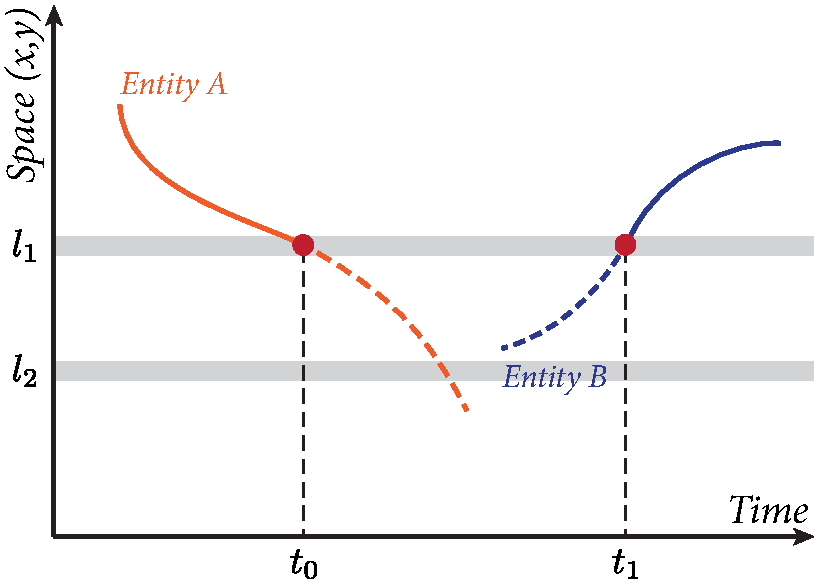
\includegraphics[width=5.3cm]{figures/dtn-indirect-async-geo.pdf}
    \caption{Indirect asynchronous composition between two entities at pre-defined locations using a \textit{stationary nodes}.}
    \label{fig:dtn-indirect-async-geo}
\end{wrapfigure}
In the previous section, we reviewed the approaches that rely on dedicated mobile relays to compose the remote movements of entities and increase the performance of the network. Conversely, other approaches leverage a collection of stationary nodes placed at strategic locations to asynchronously compose the movements of entities with intersecting trajectories. In Figure~\ref{fig:dtn-indirect-async-geo}, we represent the asynchronous composition with stationary nodes at location $l_1$ and $l_2$ that compose the trajectories of entities $A$ and $B$.

% - Placement of the stationary relays to optimize a network metric such as the delivery rate or delay
% - Forwarding of the data at the stationary nodes -> multi-path routing, replication
% - Energy-efficient communications with the entities


\paragraph{Stationary node placement.}
The main problem with this approach is to place the stationary nodes to efficiently compose the trajectories of the entities and optimize performance metrics such as the delivery rate or delay. The stationary nodes must be along the trajectories of the entities to efficiently compose their trajectories. Zhao~\etal introduced \textit{throwboxes} or small inexpensive battery-powered devices equipped with storage and wireless interfaces to enhance the delivery likelihood of mobile ad hoc networks by increasing the contact opportunities~\cite{zhao2006capacity}. The authors use linear programming models and heuristics to deploy the throwboxes based on the different knowledge they consider of the traffic matrix and the future contacts between the entities and the potential candidate locations of the throwboxes. 

In~\cite{chawathe2006inter}, Chawathe proposes to use dead drops\footnote{\url{http://deaddrops.com/}}, an art project that uses USB sticks placed at different locations in cities (\eg on the walls of buildings), to disseminate data using the opportunistic movements of vehicles to transport data from one dead drop to the other. The author proposes a placement of the dead drops using a greedy heuristic of the minimum-weight $k$-set cover problem such that it provides the required connectivity between flows of vehicles traveling different routes of interest at minimum deployment cost. 

\paragraph{Forwarding the data to the entities.}
Once the stationary nodes placed at strategic locations, the next challenge is to forward the data to the entities. With throwboxes, the authors consider different routing strategies~\cite{zhao2006capacity}. With no assumptions on the future contacts among the entities and the throwboxes, the authors propose to use the epidemic protocol between mobile entities and throwboxes. Ibrahim \etal found that allowing any forwarding interactions among the mobile entities and the intermediate nodes reduces the delivery delay of the data at the expense of additional replication~\cite{ibrahim2009analysis}. However, restricting the forwarding to the sole interactions between the mobile entities and the intermediate nodes yields poor performance in terms of delivery delay and the number of copies generated, as the source and destination must come close to an intermediate node to either transmit or receive the data. Banerjee~\etal compare the performance of forwarding strategies with two-hop (no mobile-to-mobile communications), random Epidemic (to limit the number of copies generated by message) and RAPID~\cite{balasubramanian2010replication} in the presence of different kinds of stationary intermediate nodes. The authors found that deploying $x$ base stations (connected together by an infrastructure-based network) allows reducing the average packet delay by a factor of two. The same reduction requires $2x$ mesh nodes (connected together by long range wireless links) and $5x$ relays (acting as throwboxes~\cite{zhao2006capacity}).

The forwarding problem was extensively studied in KioskNet a low-cost alternative that leverages the movements of vehicles between rural kiosks deployed in remote regions with limited Internet connectivity and offers services such as email and land records~\cite{seth2006low,guo2007very,guo2011design}. This creates a mechanical backhaul\index{mechanical backhaul} that transports data between an Internet gateway located in a nearby city and the kiosks. The kiosks serve as routers to forward the data to other kiosks, thus creating an overlay network with the kiosks as intermediate nodes and the movements of the vehicles as links. The authors propose to use different routing strategies, including flooding (does not scale), reverse-path forwarding (fragile in case of failures), and link-state routing, which uses the expected delay between two kiosks as the link weight. 

Following the same architecture as KioskNet, Demmer and Fall propose DTLSR, which modifies the \acrfullpl{lsa} with long lifetimes to take the changes in the connectivity into account~\cite{demmer2007dtlsr}. This avoids considering the node as unreachable if the link to this node is unavailable at the lime of the \acrshort{lsa} is computed, as it is the case in legacy link-state routing. The data is then routed using a shortest-path algorithm (\eg Dijkstra) such that the estimated expected delay is minimized. 

In TrainNet, the authors also formulate the routing problem of carrying data on trains as a fair resource allocation problem~\cite{zarafshan2010trainnet}. Since the trains have limited storage available and only a limited amount of data can be exchanged at stations, the routing problem maximizes the throughput and hard drive utilization, while minimizing the delay and data losses. 

\paragraph{Energy-efficient forwarding.} 
Banerjee \etal propose a framework to enable power savings at throwboxes equipped with solar panels~\cite{banerjee2007energy}. In particular, they focus on improving the neighbor discovery phase, which is the primary source of energy consumption, by using two radio channels to separate the neighbor discovery task from the data transfer task. A long-range channel is in charge of the neighbor discovery task and efficiently listens for contacts (duty-cycle), while a high-bandwidth radio remains asleep. On a contact with the long-range channel, the throwbox determines whether the contact is fruitful by (\textit{i}) predicting the future mobility of the entity and (\textit{ii}) determining whether to accommodate this contact or the future ones based on the current level of energy available and the estimated duration of this contact.

\paragraph{Combination with delivery services.}
The same approach is also used in combination with delivery services, which we introduced in Section~\ref{sec:thrid-party-services}. Wang \etal propose a centralized architecture with either a central server or geo-distributed servers~\cite{wang2004turning}. The servers aggregate the data received from parcels and dispatches it to the final users or route it across the servers, still using the postal services. Adding multiple servers allows the users to send the data to the closest server, thus reducing the costs of sending the data. Cho and Gupta propose a joint use of the Internet with postal services to minimize the cost and latency of the transfer~\cite{cho2010new,cho2011budget}. To this end, they leverage an overlay of the sites connected by both shipping links and Internet links. The overlay links are represented by a capacity, cost and transit time, which vary over time in the case of shipping links (\eg both the cost and transit time vary as a function of the level of service~---~Overnight, Two-day, Ground). The authors reduce their problem to a flow over time problem~\cite{fleischer2007quickest}, which they manage to make tractable with optimizations for large-scale networks. In every case, their system outperforms the single use of the Internet or the shipping method to transfer data. 

\paragraph{Message ferry case.}
Finally, in the case of multiple ferries, the authors propose to use a dedicated infrastructure to pass the data between ferries following different routes~\cite{zhao2005controlling}. The stationary nodes are then placed at the intersections of the ferry routes to compose the trajectories of the ferries. Bin \etal design a ferry route such that a single ferry visits the mobile entities without any online collaboration at determined locations for determined durations with a certain minimum target probability~\cite{bin2006message}. While this approach does not leverage stationary nodes, it results in an asynchronous forwarding restricted to specific locations. To design the route, the algorithm first determines the way-points among a set of candidate points and the corresponding waiting times at these way-points such that the ferry meets the other nodes with a given probability (either while moving or while waiting at a way-point). Second, the algorithms determine the route to follow such that it minimizes the weighted sum of the waiting times and the total distance of selected way-points from the center of the region.

Stationary intermediate nodes have been used in wide-range of applications and give the potential to increase the capacity of the resulting data transfers. Their placement is important to capture the trajectories of the entities to have opportunities to compose them together. This is the approach we have considered with the offloading spots to realize the offloading system we present in this thesis. 


\section{Relevance to the thesis}

In this section, we discuss the relevance of each part of our work with respect to the state-of-the-art we presented in previous sections. 

\paragraph{Vehicular data offloading.} 
In the first part of our work, we rely on offloading spots that act as intermediate relay nodes similar to those used to asynchronously compose entity trajectories at pre-defined locations such as throwboxes~\cite{zhao2006capacity}. In this case, these intermediary nodes create additional contact opportunities and bring the data closer to its destination. They also introduce non-randomness in an environment where entity trajectories are difficult to predict. The authors showed that these nodes are an effective way to compose the entity trajectories and improve the overall throughput and delivery delay.

Our system aims to transfer large amounts of delay-tolerant data, between remote locations. Examples of large data transfers over the Internet range from exchanges of large scientific datasets to distribution of high-resolution movies. Some protocols have been developed to handle bulk data transfers of several  Terabytes per day, such as GridFTP~\cite{allcock2003gridftp} or NetStitcher~\cite{laoutaris2011inter}. The latter takes into account unused bandwidth in inter-data center networks (during low link utilization periods) by using multi-path and store-and-forward scheduling at intermediate nodes for bulk transfers.

While these previous approaches allow transferring bulk data, we propose to \textit{physically offload} data by creating an alternative communication channel consisting of existing vehicle movements. Several works proposed to create such a channel by relying on the movements of entities such as airline passengers~\cite{keranen2009dtn}, trains~\cite{zarafshan2010trainnet}, or even postal services~\cite{wang2004turning,cho2011budget,laoutaris2013delay}. While these approaches are comparable with our work in terms of scale, throughput, and delay, they are difficult to compare under equivalent settings, including the number of entities involved and trips made, as well as their coverage.

\paragraph{Vehicular cloud services.}
In the case of the first extension, we rely on the schedule movements of public buses to distribute user files among repositories. This work is closely related to KioskNet~\cite{seth2006low} and DakNet~\cite{pentland2004daknet}, although they do not provide any performance evaluation and they take place in rural environments with fewer bus routes and trips available. In our system, the bus act as message ferries that connect the repositories together~\cite{zhao2004message}. While they are not controllable, they have the same purpose to connect remote nodes together.

The consumer/producer behavior of the mobile users is similar to the TierStore system, which acts as a Network File System (NFS) for applications with limited bandwidth or challenged network environments~\cite{demmer2008tierstore}. User files are stored in persistent storage repositories that lie at the core of the system (\ie static nodes similar to our repositories). Updates are applied locally at the persistent repository and distributed to other nodes. The system also uses the movements of mobile nodes to distribute updates to and from the nodes using static multicast. On the other hand, Ott and Pitk{\"a}nen proposed to use the mobile nodes to temporarily store content by means of caching~\cite{pitkanen2007redundancy,ott2007dtn} to decrease the latency when retrieving a content. This approach is similar to the one proposed by Haggle, a \textit{Pocket Switching Networking} (PSN) system that enables caching of content at intermediate nodes to also reduce the delivery delay~\cite{scott2006haggle}.

The placement of the repositories in this extension is similar to the placement of throwboxes, where the authors select the optimal locations for throwboxes from a set of candidate locations (\ie centers of square cells dividing the geographical space) to maximize the total data rate, given different knowledge on contact opportunities and traffic load for various routing strategies (\ie single-path, multi-path, and epidemic)~\cite{zhao2006capacity}. However, our placement does not account for the routing strategy, which makes it more related to the one proposed by Chawathe in the context of dead drops to disseminate data~\cite{chawathe2006inter}. In this case, the drop boxes have the same behavior as our repositories and data is disseminated using the (known) movements of vehicles. The placement of dead drops must provide the required connectivity among them at minimum deployment cost and is solved using a heuristic of the minimum-weight $k$-set cover problem fitting the model.

Finally, in the second extension, we leverage pre-defined locations selected such that vehicles encounter for a duration long enough to transfer large amounts of data through vehicle-to-vehicle communications. While these locations are similar to those used for wireless switching by Tan~\etal to create a ``vehicular backbone network''~\cite{tan2014vehicular}, or those used by Sarafijanovic-Djukic \etal to perform data forwarding~\cite{sarafijanovic2006island}, our work studies the capacity of the contacts at specific locations.

\paragraph{Logical view of the vehicle movements.}
Throughout the thesis, we analyze and characterize the vehicles' movements between locations (for the data offloading part and the first extension) or the locations where vehicles are in contact with one another (for the second extension) with a logical view representing the dynamics of the network. Our contribution lies in the fact that we use this view to translate movements into networking quantities and enable the allocation of data transfers. This is the case of the offloading overlay that mitigates the complexity of the road network and represents the flows of vehicles traveling between the offloading spots as resources to allocate. We leverage this logical view in the extensions to deploy the repositories (in the case of the first extension) and the contact hotspots (in the case of the second extension).

\paragraph{Centralized architecture.}
Instead of using a distributed control plane as is the case with most of the related approaches, we leverage a centralized architecture with a controller that has a holistic view of the system to efficiently allocate vehicular resources. In the case of the data offloading, the controller then derives forwarding states from the allocation output and installs them at the offloading spots. With these states installed, the offloading spots are able to decide which buffered data to load on the stopping vehicles. This controller performs additional management tasks, including reliable data transfers, file distribution control (in the case of the first extension), and virtual machine migrations control (in the case of the second extension).